\documentclass[10pt,a4paper]{article}
\usepackage[a4paper,margin=0.75in]{geometry}

\usepackage[T1]{fontenc}
\usepackage[icelandic]{babel}
\usepackage{lipsum}
\usepackage{natbib}

\input{../shorthandCommon}

%opening
\title{Vélabrögð} % 1000-2000 orð
\author{Helga Ingimundardóttir}

\begin{document}

\maketitle

%\begin{abstract}\end{abstract}

%\section{Inngangur}
Í stuttu máli snýst verkefnið um að læra að bera kennsl á góðar lausnir. 
Ég hef einskorðað verkefnið við tilviksrannsókn á verkniðurröðun á vélum (JSP, 
e. job-shop scheduling problem) 
sem felst í raðbundinni ákvörðunartöku um hvaða verk eigi að afgreiða næst, þar 
sem þau keppast um sömu aðföngin.
Í raun má útvíkka aðferðafræðina til hvers kyns strjála bestun. 

Hugmyndina að rannsókninni kviknaði þegar ég var að vinna í raunhæfu verkefni í 
aðgerðagreiningu í grunnnámi mínu, sem var bestun á verkniðurröðun fyrir 
Össur. Í eðli sínu er verkniðurröðun tiltölulega einfalt verkefni, sem skipar 
stóran sess hjá framleiðslufyrirtækjum, en stærðargráðan á vandamálinu gerir 
það að verkum að oft er erfitt að leysa verkefnið með nákvæmum aðferðum. 
Þetta voru mín fyrstu kynni af því að þurfa að sætta mig við einhverja lausn 
sem var ekki endilega hin fræðilega \glqq besta\grqq\ lausn. 
Hér koma brjóstvitsaðferðir (e. heuristics) eða \glqq þumalputtareglur\grqq\ 
sterkar 
inn, en þá er stóra spurningin hvernig má koma á sjálfvirkni í því ferli? 
Til að geta gert það, þá er gott að hafa skilning á því hvernig einfaldar 
reglur eru takast á við verkefnið og athuga hvort hægt sé að læra eitthvað á 
þeim áður en hafist er handa með flóknari reiknirit. 
Mun því þessi grein fjalla um gæðamat á einföldum brjóstvitsaðferðum úr 
fræðunum. 

\section*{Verkniðurröðun á vélar}
Gerum ráð fyrir að við höfum $n\times m$ JSP, 
þar sem $n$ verk, $\mathcal{J}=\{J_j\}_{j=1}^n$, 
eiga að vera afgreidd á $m$ vélum, $\mathcal{M}=\{M_a\}_{a=1}^m$. 
Verkefnin þurfa að vera afgreidd í tiltekinni röð, þ.e. sérhvert verk $J_j$ 
þarf að fylgja runu af $m$ aðgerðum 
$\vsigma_j=\{\sigma_{j1},\sigma_{j2},\dotsc,\sigma_{jm}\}$. 
Rétt er að taka fram að verk getur ekki hafist handa á næstu vél fyrr en það 
hefur lokið núverandi aðgerð. 
Þar að auki getur sérhver vél aðeins meðhöndlað/unnið eitt verk í einu. 
Viðbættar skorður sem eru oft teknar til greina eru sleppitími og skilafrestur, 
en þeir eru ekki til skoðunar hér.
Markfallið tímasetur öll verk þannig hámarks heildartími (e. makespan), 
$C_{\max}$, er lágmarkaður. 

\begin{figure}\centering
    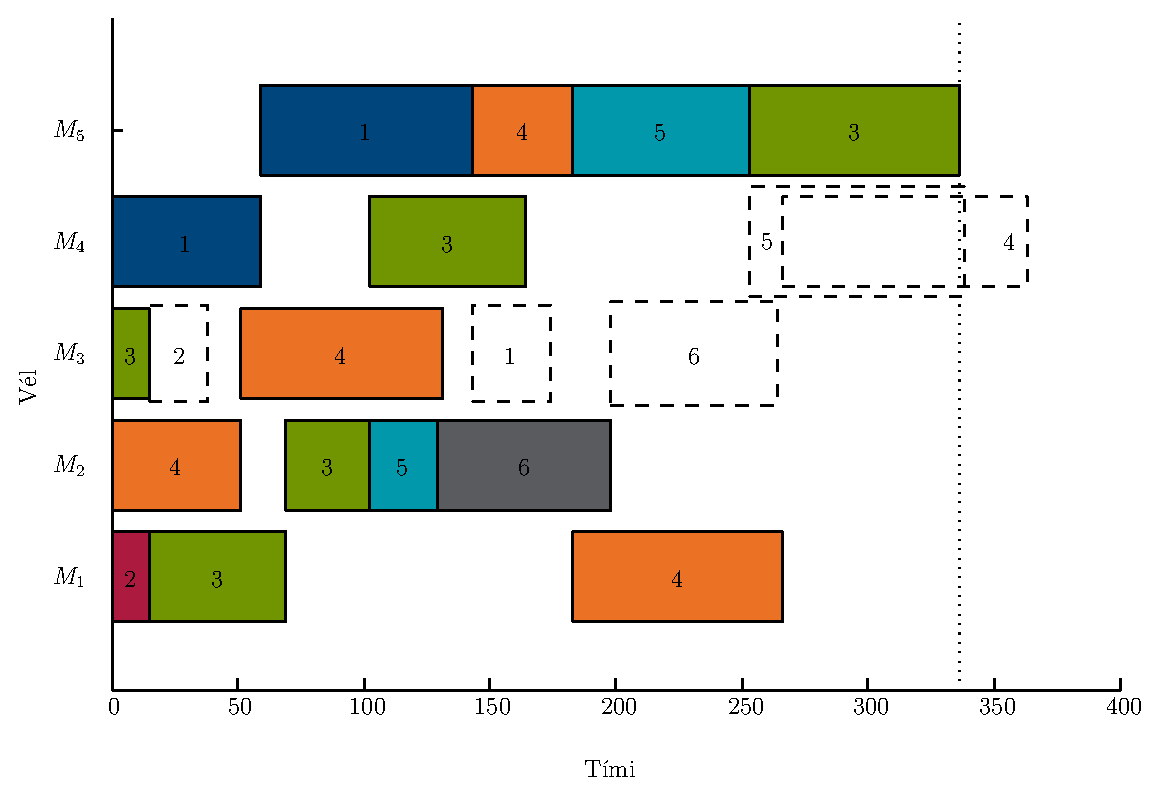
\includegraphics[width=0.5\textwidth]{figures/jssp_example.eps}
    \caption[Gantt rit af ókláraðri JSP stundaskrá]{Gantt rit af ókláraðri JSP 
    stundaskrá eftir 15 aðgerðir: heilir kassar tákna $\vchi$ og kassar með 
    brotalínu tákna $\mathcal{L}^{(16)}$. 
    Núverandi heildartími, $C_{\max}$, er gefinn upp sem punktalína.}
    \label{fig:jssp:example}
\end{figure}

Brjóstvitsaðferðir fyrir tímaáætlanir eru yfirleitt uppbyggingar- eða 
umbætunaralgrím.
Umbætunaralgrím byrjar á fullbúinni lausn og reynir að finna sambærilegar, en 
betri lausnir. 
Uppbyggingaralgrím byrjar aftur á móti með tómri lausn og bæta við einu verki í 
einu þar til lausnin er fullbúin og er það sú nálgun sem aðferðafræðin mín 
gengur út frá. 
Í þessu tilfelli þá eru yfirleitt röðunarreglur (DR, e. dispatching 
rules) sem ákvarða hvaða ókláraða verk verður valið næst. 

Það er ekki nóg að vita hvaða verkefni ætti að vera valið næst, 
heldur þarf líka að athuga hvar væri best að staðsetja það. 
Þar sem við viljum búa til samþjappaðar tímaáætlanir  þá setjum við verkið af 
stað um leið og það er laust. 
Skoðum nú Gantt ritið á mynd \ref{fig:jssp:example} sem sýnir dæmi um 
$6\times5$ JSP þar sem verknúmerið er gefið inn í kassa og er breidd þess 
vinnslutími verksins, 
vélarnar eru á lóðrétta ásinum og lárétti ásinn segir til um tíma aðgerða,
þar sem núverandi $C_{\max}$ er gefið sem punktalína. 
Búið er að setja af stað 15 aðgerðir, nefnilega, 
\begin{eqnarray}
\vchi=\left(J_3,J_3,J_3,J_3,J_4,J_4,J_5,J_1,J_1,J_2,J_4,J_6,J_4,J_5,J_3\right),
\end{eqnarray}
þar af leiðandi eru ókláruðu verkin eftirfarandi 
$\mathcal{L}=\{J_1,J_2,J_4,J_5,J_6\}$, sem lýsa þeim 5 mögulegu verkum sem geta 
verið afgreidd á tímapunkti $k=16$ (athugið að verk $J_3$ er fullklárað) -- 
þessi verk eru gefin upp með brotalínu og sýna hvernig staðan gæti breyst með 
áætlun þeirra. 
Við sjáum að $J_2$ getur verið staðsett á $M_3$ annaðhvort á milli  $J_3$ og 
$J_4$, eða eftir $J_4$.  Ef $J_6$ hefði nú þegar verið afgreitt, þá myndi 
myndast rauf á milli þess og $J_4$, þ.a.l. myndast þriðji möguleikinn, þ.e. 
fyrir $J_2$ er sett eftir $J_6$. 
Uppbyggingaralgrímið þarf því að ákveða hvert þessara raufa ætti að vera 
valið fyrir verkið og er það óháð röðunarreglunni sem er notuð. 
Mismunandi staðsetningaraðferðir geta verið skoðaðar, t.a.m. að velja þá rauf 
sem er minnsta (en nægjanlega stór) fyrir verkið. Grunnrannsóknir sýndu að 
slík nálgun gat í raun útilokað bestu lausn m.t.t. lágmarks heildartíma. 
Sú staða kemur ekki upp ef verkin eru afgreidd um leið og þau berast. 

\section*{Röðunarreglur}
Einfaldar röðunarreglur (SDR, e. single-based priority dispatching rule), er 
fall af sérkennum verka og/eða véla tímaáætlunarinnar. Sérkennin geta verið 
fastar eða breyst í takti við ákvarðanaferlið. Til dæmis getur forgangurinn 
byggst á eiginleikum vinnslutíma verkanna, til dæmis, 
\begin{description}
    \item[Stysti vinnlutími (SPT, e. shortest immediate processing time)] 
    \hfill \\ gráðug aðferð sem klárar verk með minnsta vinnslutíma fyrst. 
    \item[Lengsti vinnslutími (LPT, e. longest immediate processing time)] 
    \hfill \\ gráðug aðferð sem klárar verk með stærsta vinnslutíma fyrst. 
    \item[Minnsta heildarvinna (LWR, e. least work remaining)] \hfill \\
    þar sem ásetningurinn er að klára verk sem eru komin langt á veg í 
    framvindu sinni, þ.e. að lágmarka verklistann $\mathcal{L}$.
    \item[Mesta heildarvinna (MWR, e. most work remaining)] \hfill \\
    þar sem ásetningurinn er að flýta fyrir framvindu verka sem krefjast mikinn 
    vinnslutíma og gefur því af sér jafnari framvindu fyrir öll verk.
\end{description}
Þetta eru þær algengustu röðunarreglur í starfi vegna einfaldleika þeirra og 
skilvirkni, en ótal fleiri reglur koma til greina. Yfirlit yfir 100 
sígildar röðunarreglur má finna í \citet{Panwalkar77}, einnig er greinargóð 
lýsing á SDR eftir \citet{Haupt89}. 

\section*{Tilraunir}
Skoðum nú tvær gagnadreifingar fyrir JSP, slembin
uppröðun, kölluð \texttt{j.rnd}, og einsleit uppröðun, kölluð \texttt{f.rnd}. 
Vinnslutíminn í báðum tilfellum er fengin með jafnri dreifingu á bilinu 
$[1,99]$.
Við höfum $N_{\textbf{train}}=500$ af hvorri dreifingu og vitum bestu lausn 
með því að besta með hugbúnaði fyrir línuleg bestunarverkefni. 

Þar sem vinnslutíminn er mismunandi þá munum við styðjast við að lágmarka 
frávik frá bestu lausn með eftirfarandi hætti, 
\begin{equation}
\rho=\frac{C_{\max}^{\text{DR}}-C_{\max}^{\text{opt}}}{C_{\max}^{\text{opt}}}
\cdot 100\%
\end{equation}
þar sem $C_{\max}^{\text{DR}}$ er fengið með DR og $C_{\max}^{\text{opt}}$ er 
besta lausn. 

Nú eru SDR sem voru kynntar ááðan notaðar á  gagnasettin. Kassarit fyrir 
$\rho$ er gefið upp í mynd \ref{fig:boxplot}. Við sjáum að það er greinilegur 
munur á því hvaða SDR er beitt á gögnin, t.a.m. er MWR mjög hentug regla fyrir 
\texttt{j.rnd}, aftur á móti er það ekki tilvikið fyrir \texttt{f.rnd} þar sem 
gagnstæð regla, LWR, kemur umtalsvert betur út. 

\begin{figure}\centering
    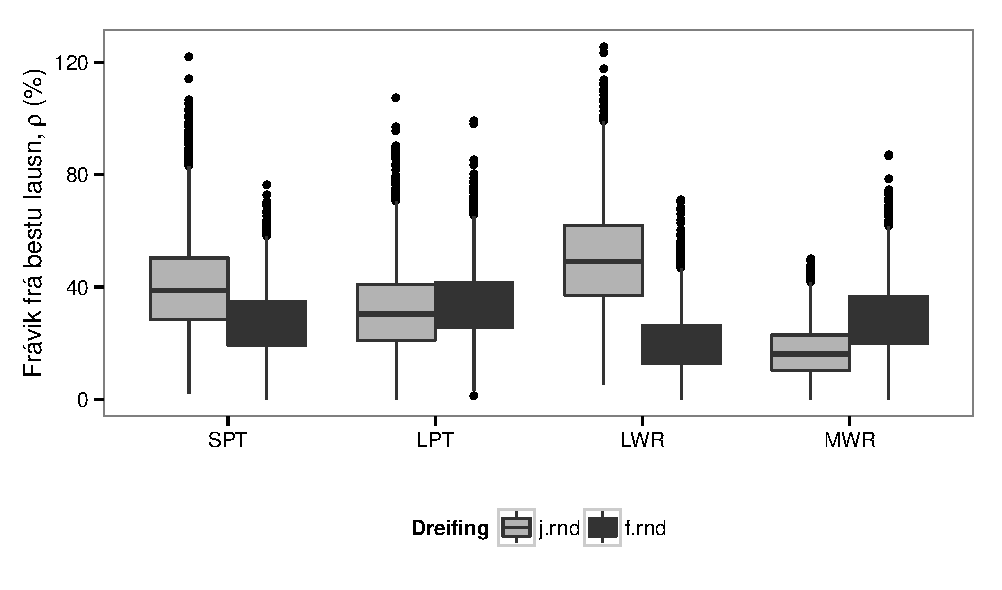
\includegraphics[width=0.5\textwidth]{figures/boxplot.pdf}
    \caption{Kassarit fyrir SDR}
    \label{fig:boxplot}
\end{figure}

Í mörgum tilfellum þá er látið staðar numið við þessar niðurstöður og sú DR sem 
kom best út er valin fyrir verkefnið. En það sem við viljum vita er hvað 
aðgreinir þessar reglur? Af hverju er svona mikill munur á niðurstöðum? 
Sérstaklega í ljósi þess að innblástur þeirra virðist ekki vera svo ólíkur; 
SPT svipar til LWR og LPT til MWR. Einnig er SPT andstæða LPT og LWR fyrir MWR. 
Af hverju er einsleit verkumröðun \texttt{f.rnd} að velja LWR fram yfir MWR og 
öfugt? Einnig hvenær fer að greina á gæði lausnanna með þessum aðferðum?

Ef við skoðum bestu lausnir fyrir verkefnin og athuga hvenær þær væru 
jafngildar að beita SDR, líkt og mynd \ref{fig:diff:opt:SDR} sýnir, þá fyrir 
\texttt{j.rnd} má sjá að oftar en ekki er LWR og LPT verri en að velja verk að 
handahófi sé best (brotalína), sem útskýrir slakar niðurstöður þeirra. 
Einnig má sjá að SPT sýnir hegðun sem er líklegri til að 
hagstæðri en MWR -- en aðeins til að byrja með. Eftir það fer MWR að vera 
líklegri til vinnings. En því miður er ekki hægt að beita SPT fyrst (segjum frá 
skrefi 1-10) og láta svo MWR taka svo við, því þá erum við nú þegar búin að 
stilla tímaáætluna á þann veg að MWR nær ekki að rétta sig af. 

\begin{figure}\centering
    \includegraphics[width=0.5\textwidth]{figures/{stepwise.6x5.OPT.SDR}.pdf}
    \caption{Líkurnar að SDR sé hagstæðust, brotalínan lýsir að verk að 
    handhófi sé hagstæðast.}
    \label{fig:diff:opt:SDR}
\end{figure}

Deila má hvert þetta sé nægjanlegur samanburður. Því það sem verið er að gera 
hér er að \glqq elta\grqq\ bestu lausn og reyna að skoða \emph{eftir á} hvernig 
hefði mátt velja samsvarandi SDR sem hefði gefið sömu lausn, úr \emph{bestu} 
stöðu. 
Vandamálið felst einna helst í því að um leið og \glqq röng\grqq\ ákvörðun þá 
er byrjað að afvegaleiða lausnina í ástandsrúminu.
Því skiptir máli að lágmarka afleiðingu þess í hvert sinn, þar sem yfirleitt 
eru gerðar ítrekað rangar ákvarðanir. Þá skiptir máli, að velja 
a.m.k. \glqq góðar\grqq\ rangar ákvarðanir.

Ef við skoðum nú hvernig eru reglurnar að breytast frá öðrum verkum sem eru 
ekki valin? Með öðrum orðum, sambærilegt og áður í mynd \ref{fig:diff:opt:SDR}, 
nema nú eltum við SDR í stað bestu lausnar. 
Mynd \ref{diff:case:track:6x5} sýnir hvernig frávikið á $\rho$ er 
að breytast sem fall af ákvörðunarskrefi með því að fylgja ákveðinni SDR 
(brotalína). Einnig er skoðað hvernig besta og versta frávik væri frá þeirri 
sömu stöðu, þ.e. ef við fylgdum ekki reglunni. 
Þá sést glögglega að MWR er stöðugt að ná betri stöðu en SPT, 
jafnvel þótt bestu lausnirnar virtust fylgja SPT hegðun til að byrja með. 

Með því að líta á frávikin frá reglunum, þá eru augljóslega tækifæri að 
betrumbæta reglurnar upp á einhverju marki, þ.e. þegar besta frávik er lægra 
heldur en að fylgja reglunni. Þetta stenst við fræðin, því ef vandað er til 
verks þá eru samsettar röðunarreglur (CDR, e. composite dispatching rules)  
iðulega betri en þær einar og sér \citep{Jayamohan04}. 

\begin{figure}\centering
    \includegraphics[width=0.5\textwidth]{figures/{stepwise.6x5.Track.casescenario}.pdf}
    \caption{Breyting frávik sem fall af áætlunarskrefi fyrir gefið SDR.}
    \label{diff:case:track:6x5}
\end{figure}

\citet{Siggi05} hafa til að mynda notað ákvarðanatré til að læra LPT fyrir 
JSP. 
Vankanturinn þar var sá að þá var verið að reyna að læra regluna án þess að 
umbuna þau frávik sem hefðu leitt til betri niðurstöður. 
Væri því rökrétt að læra frekar af væntri niðurstöðu, þ.e. afleitt $C_{\max}$ 
fyrir gefna ákvörðun m.t.t. bestu lausnar, líkt og gert var síðar í 
\cite{Malik08,Russell09} og \cite{Siggi10}. Þannig má finna CDR sem betrumbætir 
LPT regluna sem hún byggist á. 
Slík var nálgunin hjá mér í \cite{InRu15a}, þar 
sem skoðuð voru 13 sérkenni JSP lausna, sem innblástur var mikið til sóttur til 
sígildra SDR. Þar var framkvæmdur forgangslærdómur (e. preference learning) 
til að finna línulegt fall sérkenna byggt á þjálfunargögnum þar sem stöður sem 
leiddu af sér hagstæðra $C_{\max}$ voru teknar fram yfir óhagstæðari. 
Niðurstöður leiddu í ljós að það gott að búa til módel sem byggjast á bestu 
lausnum. Aftur á móti geta þjálfunargögnin verið einsleit og þar af leiðandi 
ekki nægjanlega lýsandi fyrir ástandsrýmið. 
Þá var brugðið á það ráð að bæta við þjálfunargögnum sem byggðust á 
góðum SDR til að veita meiri fjölbreytileika til að læra af og til að takast á 
við að festast í staðbundnu lággildi, með góðum niðurstöðum. 
Mögulega er breytileikinn á milli gagna of mikil með slíkri nálgun. 
Núverandi rannsóknir ganga út á eftirlíkingarlærdóm (e. imitation learning) í 
anda \cite{RossB10} og \cite{RossGB11} þar sem búið er til módel sem lærir 
forgang af bestu braut (sbr. \cite{InRu11a,InRu15a}), sem er síðan notað til að 
búa til ný þjálfunargögn. 
Þetta er gert á endurkvæman hátt, þar sem í hverri ítrun nær módelið að 
endurspegla þjálfunargögnin betur og betur. 
Fyrstu niðurstöður liggja fyrir og ýtir aðferðin uppá við afköst núverandi 
aðferðafræði. 

%          Problem Dimension    Q1    Q3
%          j.rnd       6x5 19.91 47.21
%          f.rnd       6x5 18.46 35.52

\bibliographystyle{unsrtnat}
\begin{thebibliography}{11}
    \providecommand{\natexlab}[1]{#1}
    \providecommand{\url}[1]{\texttt{#1}}
    \expandafter\ifx\csname urlstyle\endcsname\relax
    \providecommand{\doi}[1]{doi: #1}\else
    \providecommand{\doi}{doi: \begingroup \urlstyle{rm}\Url}\fi
    
    \bibitem[Panwalkar and Iskander(1977)]{Panwalkar77}
    S.~S. Panwalkar and Wafik Iskander.
    \newblock A survey of scheduling rules.
    \newblock \emph{Operations Research}, 25\penalty0 (1):\penalty0 45--61, 
    1977.
    
    \bibitem[Haupt(1989)]{Haupt89}
    R.~Haupt.
    \newblock A survey of priority rule-based scheduling.
    \newblock \emph{OR Spectrum}, 11:\penalty0 3--16, 1989.
    
    \bibitem[Jayamohan and Rajendran(2004)]{Jayamohan04}
    M.S. Jayamohan and Chandrasekharan Rajendran.
    \newblock Development and analysis of cost-based dispatching rules for job 
    shop
    scheduling.
    \newblock \emph{European Journal of Operational Research}, 157\penalty0
    (2):\penalty0 307--321, 2004.
    
    \bibitem[Li and Olafsson(2005)]{Siggi05}
    Xiaonan Li and Sigurdur Olafsson.
    \newblock Discovering dispatching rules using data mining.
    \newblock \emph{Journal of Scheduling}, 8:\penalty0 515--527, 2005.
    
    \bibitem[Olafsson and Li(2010)]{Siggi10}
    Sigurdur Olafsson and Xiaonan Li.
    \newblock Learning effective new single machine dispatching rules from 
    optimal
    scheduling data.
    \newblock \emph{International Journal of Production Economics}, 128\penalty0
    (1):\penalty0 118--126, 2010.
    
    \bibitem[Malik et~al.(2008)Malik, Russell, Chase, and Beek]{Malik08}
    Abid~M. Malik, Tyrel Russell, Michael Chase, and Peter Beek.
    \newblock Learning heuristics for basic block instruction scheduling.
    \newblock \emph{Journal of Heuristics}, 14\penalty0 (6):\penalty0 549--569,
    December 2008.
    
    \bibitem[Russell et~al.(2009)Russell, Malik, Chase, and van Beek]{Russell09}
    Tyrel Russell, Abid~M. Malik, Michael Chase, and Peter van Beek.
    \newblock Learning heuristics for the superblock instruction scheduling
    problem.
    \newblock \emph{IEEE Trans. on Knowl. and Data Eng.}, 21\penalty0
    (10):\penalty0 1489--1502, October 2009.
    
    \bibitem[Ingimundardottir and Runarsson(2015)]{InRu15a}
    Helga Ingimundardottir and Thomas~Philip Runarsson.
    \newblock Generating training data for supervised learning linear composite
    dispatch rules for scheduling.
    \newblock In \emph{9th international conference on Learning and Intelligent
        Optimization (LION'09)}, 2015.
    
    \bibitem[Ross and Bagnell(2010)]{RossB10}
    Stéphane Ross and Drew Bagnell.
    \newblock Efficient reductions for imitation learning.
    \newblock In Yee~W. Teh and D.~M. Titterington, editors, \emph{Proceedings 
    of
        the Thirteenth International Conference on Artificial Intelligence and
        Statistics (AISTATS-10)}, volume~9, pages 661--668, 2010.
    
    \bibitem[Ross et~al.(2011)Ross, Gordon, and Bagnell]{RossGB11}
    Stéphane Ross, Geoffrey~J. Gordon, and Drew Bagnell.
    \newblock A reduction of imitation learning and structured prediction to
    no-regret online learning.
    \newblock In Geoffrey~J. Gordon and David~B. Dunson, editors, 
    \emph{Proceedings
        of the Fourteenth International Conference on Artificial Intelligence 
        and
        Statistics (AISTATS-11)}, volume~15, pages 627--635. Journal of Machine
    Learning Research - Workshop and Conference Proceedings, 2011.
    
    \bibitem[Ingimundardottir and Runarsson(2011)]{InRu11a}
    Helga Ingimundardottir and Thomas~Philip Runarsson.
    \newblock Supervised learning linear priority dispatch rules for job-shop
    scheduling.
    \newblock In Carlos Coello, editor, \emph{Learning and Intelligent
        Optimization}, volume 6683 of \emph{Lecture Notes in Computer Science}, 
        pages
    263--277. Springer, Berlin, Heidelberg, 2011.
    
\end{thebibliography}

\end{document}
